\section{The Sybil attack}

In this section we will explain the Sybil attack\cite{douceur-sybil}
and how it can be used in the MultiChain system to create an artificial reputation.
An universallly applicable solution has not yet be found\cite{levine-sybilsurvey}.

\subsection{Using fake indentities}
In large distributed systems convincingly distinct identities can be presented
that are infact all under the control of a single adversary M.
Identities can be public keys like in the Dispersy system
or other abstractions of information without direct physical knowledge.
These identities can participate in the system acting like normal agents,
but they can also help each other malificiently to boost each other towards a common goal.

In the MultiChain system the attack is done in the following way.
M creates several other identities besides his own.
This involves generating several key pairs.
Now M controls several identities that can be presented convincingly.
The key pairs do not have to be linked to a node responding to requests.
Failure of nodes are typical in large distributed systems.

Using these key pairs M can now generate an artificial reputation.
Transactions between M and the fake identities are generated by M.
These are signed using the keys of the fake identities.
Using a single transaction it cannot be determined if it is between two distinct identities or a single distinct identity and a fake identity.

\begin{figure}
	\centerline{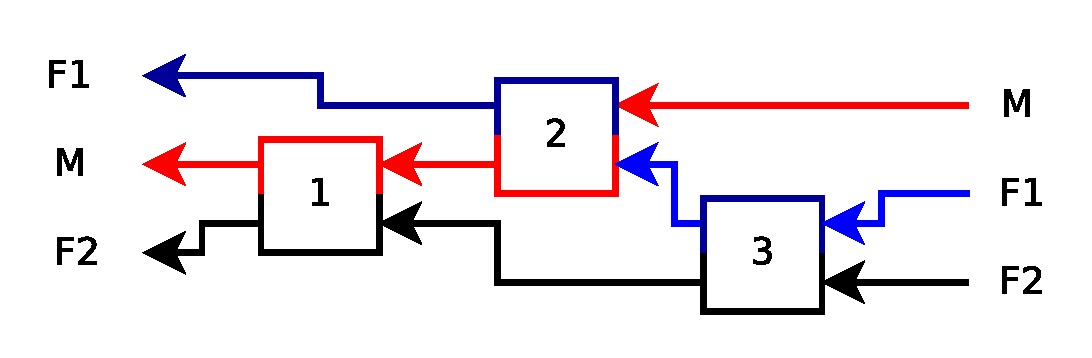
\includegraphics[scale=0.3]{problems/figs/sybil.eps}}
	\caption{The sybil attack by M.}
	\label{fig:sybil-example}
\end{figure}

An example of the Sybil Attack can be seen in \ref{fig:sybil-example}.
In this example M is the malificient node and F1 and F2 his fake identities.
Block 1 and block 2 contain a transaction that is favourable to M,
but M has done nothing to deserve these.
Similair blocks like block 3 can be generated between fake identities in an effort to thwart efforts to analyse the network
and detect fake identities.

In this way M is able to boost his reputation without much work.
The more sophisticated the generation is done by M,
the harder it will be to detect that M boosted his reputation using fake identities.
M can then abuse his fake reputation by solliciting cooperation from other nodes in the network.
They will respond positively on the request by M based upon the false reputation M claims to have.

\subsection{Validating Identities}
A node can have three potential sources of validation of distinct identities:
\begin{itemize}
\item Itself
\item Other entitites
\item A trusted, central authority
\end{itemize}

A node itself could try to directly validate two identities to be distinct.
It would challenge several identities to complete a task that only two entities could complete.
The task would require more resources then a single entity possesses and will be issued simultaneously to all identities.
If the identities complete the task, they have proven to be distinct.
Example of required resources are communication, storage and computation.
These challenges can scale to validate more entities at once.

Indirect validation can be used by a node to by delegating validation to other entities.
A node could accept additional identities to be distinct when an accepted identity vouches for it.
The node has the delegated responsibility to challenge the entity with a challenge.
This would limit the total amount of challenges needed.
But an obvious pitfall of delegating this to other identities is that these can vouch for fraudelent identities.
Next to this, it involves an increase in complexity as the challenges still have to be issued concurrently.

But these challenges are highly indesirable.
These challenges require by definition to occupy between two nodes a limited resource to the maximum capacity of a single node.
While not providing any additional functionality beyond asserting distinct identities.
These challenges also prove inworkable when entities have hugely different amount of resources available.
No challenge can be constructed that can be worked by less powerfull devices,
that could not be worked several times by more powerfull devices.

Next to this, these challenges are only usable with nodes that are active and responding to challenges.
If a node becomes inactive it cannot be ascertained if the node is a fake identity.
But this identity still makes claim about a reputation of another entity.
A choice has to be made between either not counting these claims and allow for a drop in reputation of a node or
allow claims that cannot be validated to be taken into account.
Both options lower the usability of the system.

A trusted, central authority would be able to vouch for distinct indentities
if it has an other way outside the system of asserting that it indeed is a distinct identity.
Approaches exists that implicitly rely on the authority of a trusted agency.
But a central authority goes against the principles of a peer-to-peer network.

Several other defenses against the Sybil Attack have been proposed\cite{newsome-sybil}\cite{dinger-sybil}
or variants on the defenses stated here\cite{levine-sybilsurvey}.
But these either have the same limitation and are minor improvements or are non-applicable for MultiChain.

\subsection{Possibility of attack and likelyhood of detecting fraud}
For M to conduct the Sybil Attack he will need to generate a set of key pairs.
This is trivial to do and Dispersy provides functionality to do this very easily.

\todo{Timing of generating several keys}

With these keys M has to generate blocks.

\todo{timing of generating blocks}

Sybil Attack can have a wide range of sophistication.
Ranging from a large amount of fake identities with a large amount of transaction between them
to a single, fake identity boosting the reputation of M in a couple of transaction.
Even these simple Sybil Attack are hard to defend against if these are not done to obviously.